\documentclass[10pt,twocolumn,letterpaper]{article}
\usepackage{times}
\usepackage{microtype}
\usepackage{graphicx}
\usepackage{booktabs}
\usepackage{array}
\usepackage{multirow}
\usepackage{url}
\usepackage{amsmath}
\usepackage{amssymb}
\usepackage{enumitem}
\usepackage{xcolor}
\usepackage{float}
% CVPR two-column page geometry, folded into this standalone source.
\setlength{\paperheight}{11in}
\setlength{\paperwidth}{8.5in}
\setlength{\textheight}{8.875in}
\setlength{\textwidth}{6.875in}
\setlength{\columnsep}{0.3125in}
\setlength{\topmargin}{-0.25in}
\setlength{\headheight}{0in}
\setlength{\headsep}{0in}
\setlength{\oddsidemargin}{-0.1875in}
\setlength{\evensidemargin}{-0.1875in}
\definecolor{cvprblue}{rgb}{0.21,0.49,0.74}
\usepackage[breaklinks,colorlinks,allcolors=cvprblue]{hyperref}
\setlength{\textfloatsep}{5pt plus 1pt minus 1pt}
\setlength{\floatsep}{4pt plus 1pt minus 1pt}
\setlength{\intextsep}{5pt plus 1pt minus 1pt}
\setlength{\abovecaptionskip}{3pt}
\setlength{\belowcaptionskip}{0pt}
\setlist{nosep,leftmargin=*}
\newcommand{\pct}[1]{#1\%}
\newcommand{\NA}{\textit{None}}

\def\confName{Machine Learning}
\def\confYear{2026}
\title{Trees, Bagging, and Multiclass Boosting on Olivetti Faces}
\author{Jiya Yadav\\Roll number: M26CSE004\\
\small Submission repository: included in \texttt{Jiya\_Yadav\_M26CSE004\_Assignment2.zip}\\
\small Code snapshot: \texttt{0679161a6a89}}

\begin{document}
\maketitle

\begin{abstract}
I studied decision trees, bootstrap bagging, and SAMME boosting on the 40-person Olivetti faces data. The split was made separately inside each identity, so every person contributed six training images, two validation images, and two test images. A single unpruned tree reached \pct{53.75} clean test accuracy. Bagging 100 copies of that tree raised it to \pct{85.00} and remained much stronger after the centre of each test face was removed. Boosting behaved differently: it kept returning to a small set of hard training faces, but the selected model did not match bagging on this data. Thirty resampled training sets make the difference clear. Bagging sharply reduced variance while keeping useful depth; a shallow tree had little variance to remove but too much bias.
\end{abstract}

\section{Data and common setup}
The seed is 26004, obtained by reading the numeric characters of M26CSE004 in order. I used \texttt{fetch\_olivetti\_faces} without shuffling the source data, then applied one seeded permutation inside each identity. The saved split contains 240 training, 80 validation, and 80 test images. Inputs are the raw $64\times64$ pixels flattened to 4096 numbers. No scaling, PCA, or feature selection was used. For the second test set I set rows 24 to 39 and columns 24 to 39 to zero. Every model was trained on clean faces only.

All choices were made from clean validation accuracy. When settings tied exactly, I used the smaller ensemble and the less fragile tree setting. The test set and its masked copy were opened only after the choices were frozen. Labels below are the integer identities 0 through 39 returned by scikit-learn.

\section{Single tree and bagging}
\subsection{Choosing the tree}
I trained all 15 requested depth and leaf-size combinations. Table~\ref{tab:tree} shows the leaf-size-two row at every depth because it also contains the selected setting; the complete grid is saved as \texttt{results/tree\_grid.csv}. Leaf sizes one, two, and four were identical through depth 16. At unlimited depth, leaf sizes one and two tied at \pct{51.25} validation accuracy, while leaf size four fell to \pct{47.50}. I kept leaf size two because it removed the singleton leaves without lowering validation accuracy.

\begin{table}[t]
\centering
\caption{Tree results for \texttt{min\_samples\_leaf=2}. Accuracies are percentages. $\bar n$ is the mean number of training examples in an occupied leaf and $f_1$ is the fraction of leaves containing one training example.}
\label{tab:tree}
\scriptsize
\begin{tabular}{r@{\hspace{5pt}}rrrrrr}
\toprule
Depth & Train & Val. & Test & Leaves & $\bar n$ & $f_1$\\
\midrule
2 & 7.50 & 6.25 & 7.50 & 3 & 80.00 & 0\\
4 & 12.50 & 8.75 & 8.75 & 5 & 48.00 & 0\\
8 & 22.50 & 16.25 & 18.75 & 9 & 26.67 & 0\\
16 & 44.58 & 23.75 & 28.75 & 18 & 13.33 & 0\\
\NA & 97.08 & \textbf{51.25} & 53.75 & 47 & 5.11 & 0\\
\bottomrule
\end{tabular}
\end{table}

Depth changes what the tree can separate. The depth-two tree makes only three occupied leaves for 40 identities, so most classes are forced together. More depth steadily lowers this restriction, but it also makes smaller leaves. The unlimited leaf-size-one tree went all the way to \pct{100} training accuracy and had \pct{14.89} singleton leaves. Leaf size two gave nearly the same fit without those one-image rules.

\subsection{Bagging from bootstrap samples}
For each tree I drew 240 training positions with replacement and fit the frozen tree setting. Prediction is an unweighted class vote. Table~\ref{tab:bag} uses prefixes of the same 200-tree sequence. A bootstrap sample contained about 152 distinct faces, almost exactly the finite-sample expectation
\begin{equation}
240\left[1-\left(1-\frac{1}{240}\right)^{240}\right]=151.89.
\end{equation}

\begin{table}[t]
\centering
\caption{Bagging results. $U$ is the mean number of distinct faces in a bootstrap sample.}
\label{tab:bag}
\scriptsize
\begin{tabular}{r@{\hspace{5pt}}rrrrr}
\toprule
$B$ & Train & Val. & Test & $U$ & OOB\\
\midrule
1 & 67.92 & 43.75 & 46.25 & 136.00 & 30.77\\
5 & 92.92 & 62.50 & 66.25 & 150.60 & 28.50\\
10 & 99.58 & 73.75 & 73.75 & 152.10 & 41.35\\
25 & 100 & 87.50 & 83.75 & 151.76 & 60.42\\
50 & 100 & 85.00 & 86.25 & 152.54 & 71.67\\
100 & 100 & \textbf{88.75} & 85.00 & 152.18 & 75.42\\
200 & 100 & \textbf{88.75} & 85.00 & 152.15 & 78.33\\
\bottomrule
\end{tabular}
\end{table}

The 100-tree and 200-tree models tied on validation accuracy, so I froze $B=100$. The first OOB figure is noisy because only \pct{43.33} of training faces receive an OOB vote at $B=1$. Coverage reaches \pct{100} at $B=25$.

\begin{figure}[t]
\centering
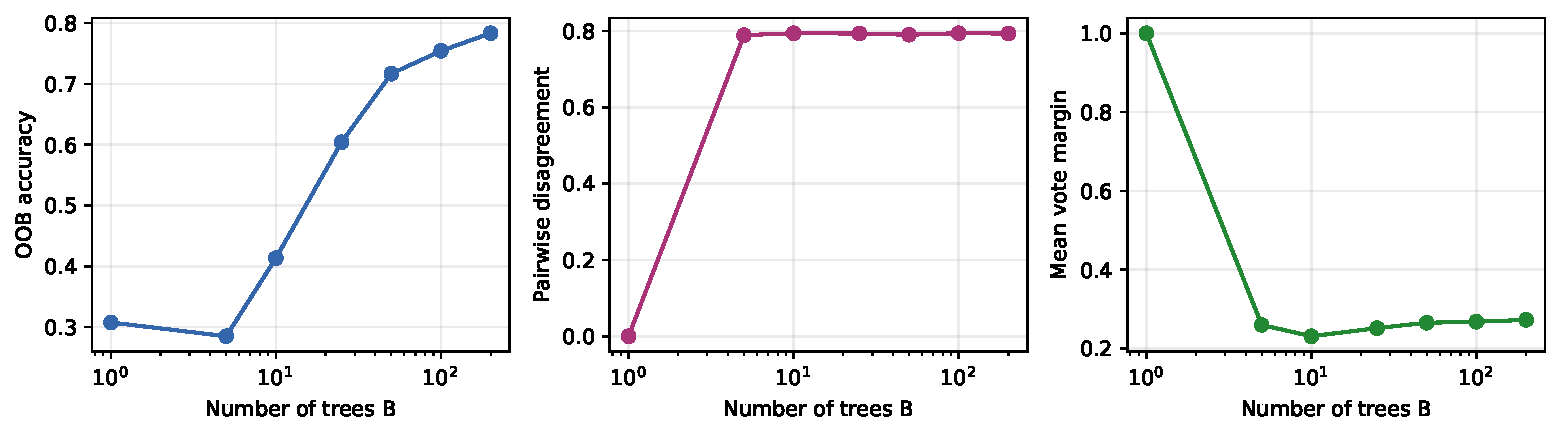
\includegraphics[width=\linewidth]{../figures/bagging_metrics.pdf}
\caption{OOB accuracy, validation-set tree disagreement, and validation vote margin for bagging prefixes.}
\label{fig:bagmetrics}
\end{figure}

Figure~\ref{fig:bagmetrics} explains why adding trees first helps and then settles. Pairwise disagreement stays close to 0.79. This is useful diversity rather than a sign that the vote is failing: the mean margin rises from 0.23 at ten trees to 0.27 at 100, while OOB accuracy keeps improving. After 100 trees, the validation prediction no longer changes.

\subsection{Clean and masked faces}
\begin{table}[t]
\centering
\caption{Frozen tree and bagging model. Confidence is the winning class probability for the tree and the winning vote fraction for bagging.}
\label{tab:q1mask}
\scriptsize
\begin{tabular}{llrr}
\toprule
Test set & Model & Accuracy & Confidence\\
\midrule
\multirow{2}{*}{Clean} & Tree & 53.75 & 96.25\\
 & Bagging & 85.00 & 41.13\\
\midrule
\multirow{2}{*}{Masked} & Tree & 18.75 & 100.00\\
 & Bagging & 68.75 & 27.18\\
\bottomrule
\end{tabular}
\end{table}

The single tree is very sure even when it is wrong. Masking cuts its accuracy by 35 points while its mean confidence rises to one, an effect of landing in pure terminal leaves. Bagging loses 16.25 points and its vote becomes less concentrated, which is a more honest response to missing pixels.

\begin{figure}[t]
\centering
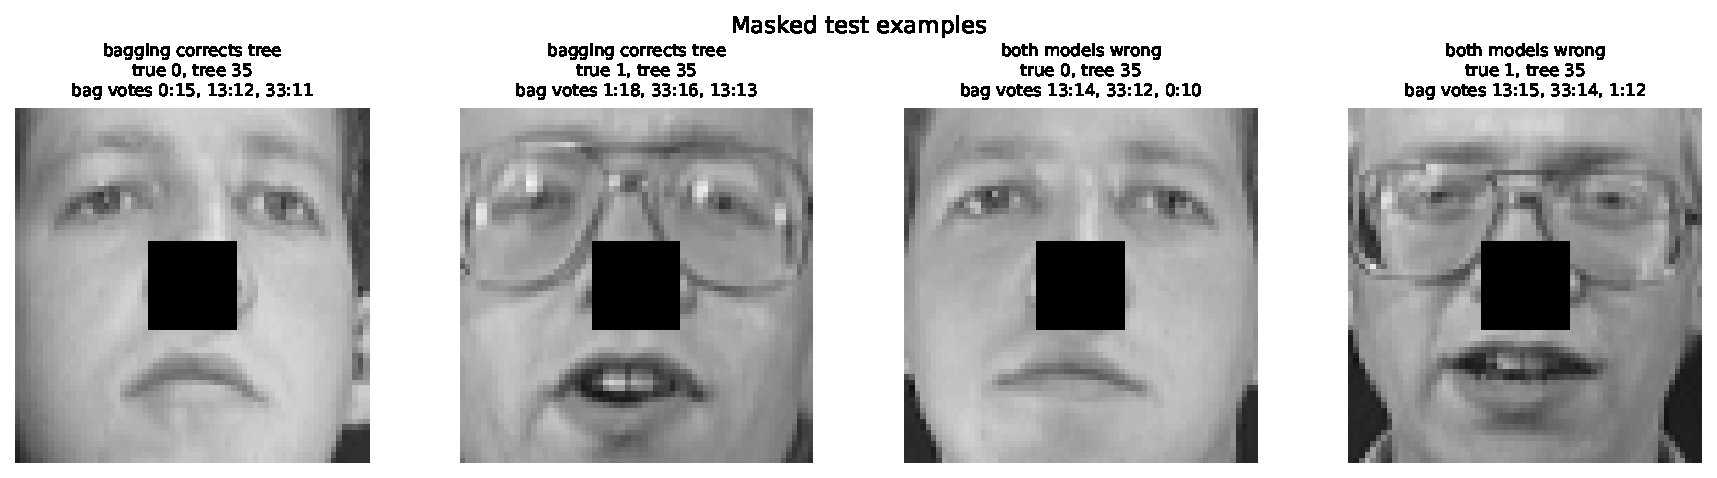
\includegraphics[width=\linewidth]{../figures/bagging_examples.pdf}
\caption{Two masked faces where bagging corrects the tree and two where both are wrong. The three largest nonzero vote counts are printed above each face.}
\label{fig:bagfaces}
\end{figure}

On test faces 8 and 14 (source indices), the tree sends both examples to class 35. Bootstrap trees split across several plausible classes, but the correct classes 0 and 1 win with 15 and 18 votes. This is the kind of unstable boundary error that averaging can fix. For source indices 6 and 16, class 13 wins while the correct class is a close runner-up. Many trees make the same mistake after the central evidence is removed. Voting cannot repair a shared blind spot.

\section{Multiclass boosting from scratch}
\subsection{One complete SAMME round}
I first checked the update on nine ordered points with three classes. A depth-one tree predicts $[1,1,1,1,1,2,2,2,2]$ for targets $[0,0,1,1,1,2,2,2,0]$. Three points are wrong, so $\epsilon=1/3$ and
\begin{equation}
\alpha=\log\frac{1-1/3}{1/3}+\log(3-1)=1.3863.
\end{equation}

\begin{table}[t]
\centering
\caption{The complete toy SAMME round. All initial weights are $1/9$.}
\label{tab:toy}
\scriptsize
\begin{tabular}{rrrrrr}
\toprule
$i$ & $x$ & $y$ & $h(x)$ & Wrong & New weight\\
\midrule
1&0&0&1&1&0.2222\\
2&1&0&1&1&0.2222\\
3&2&1&1&0&0.0556\\
4&3&1&1&0&0.0556\\
5&4&1&1&0&0.0556\\
6&5&2&2&0&0.0556\\
7&6&2&2&0&0.0556\\
8&7&2&2&0&0.0556\\
9&8&0&2&1&0.2222\\
\bottomrule
\end{tabular}
\end{table}

The three misses receive four times the weight of a correct point after normalisation. The face-data code uses this same update. If a learner has $\epsilon\geq1-1/K$, it is not added; if its error is numerically zero, the error is clipped for a finite weight and fitting stops.

\subsection{Selecting depth and rounds}
Table~\ref{tab:boostgrid} gives clean validation accuracy for all 16 choices. Depth three with 50 rounds and depth four with 100 rounds both reach \pct{35}. I chose 50 rounds because the validation score was already tied there. The frozen model has \pct{72.08} training accuracy and \pct{28.75} clean test accuracy.

\begin{table}[t]
\centering
\caption{SAMME validation accuracy (percent).}
\label{tab:boostgrid}
\scriptsize
\begin{tabular}{r@{\hspace{8pt}}rrrr}
\toprule
Depth & 10 & 25 & 50 & 100 rounds\\
\midrule
1 & 3.75 & 8.75 & 13.75 & 8.75\\
2 & 7.50 & 13.75 & 18.75 & 12.50\\
3 & 15.00 & 17.50 & \textbf{35.00} & 28.75\\
4 & 10.00 & 16.25 & 28.75 & \textbf{35.00}\\
\bottomrule
\end{tabular}
\end{table}

\begin{figure}[t]
\centering
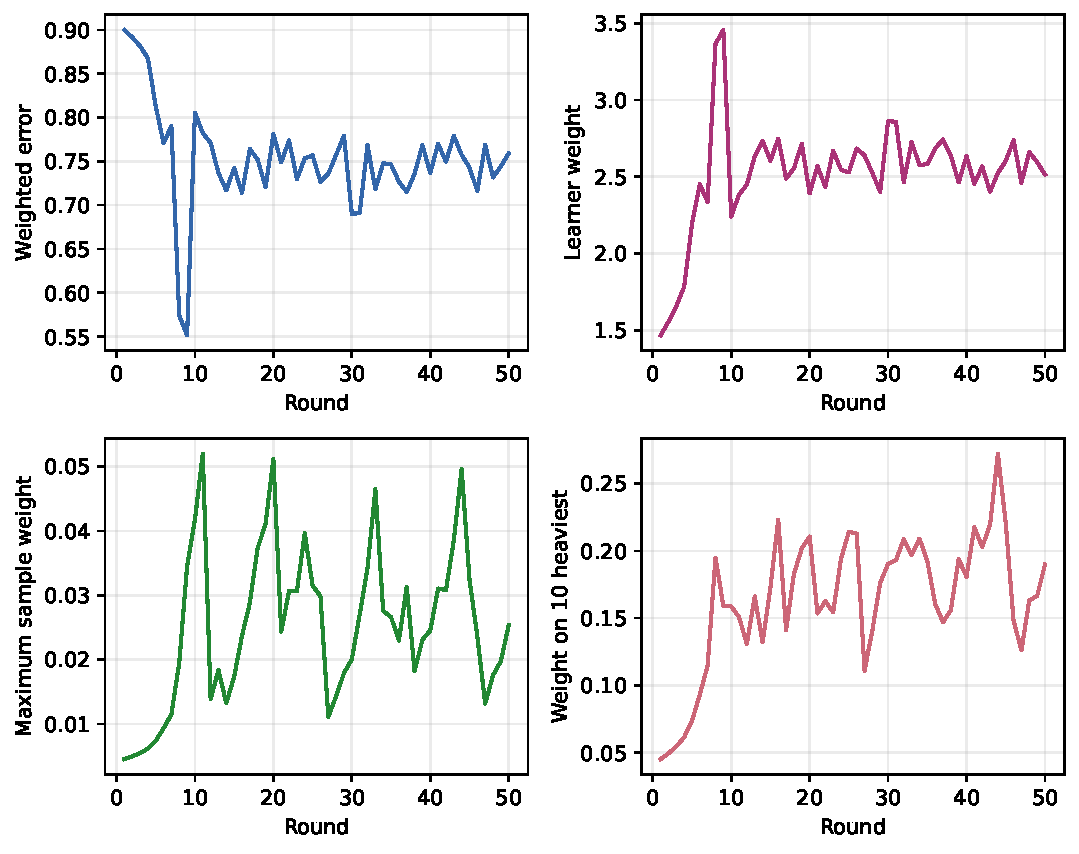
\includegraphics[width=0.92\linewidth]{../figures/boosting_dynamics.pdf}
\caption{Selected SAMME run. The learner error and weight move from round to round as hard images receive more mass.}
\label{fig:boostdyn}
\end{figure}

At round 50, the current learner's weighted error is 0.7592, safely below the 40-class random threshold of 0.975. Its weight is 2.515. The largest image weight is 0.0253, and the ten heaviest images carry 0.1898 in total. The curve is not monotone because each new tree changes the distribution that the next tree sees.

\subsection{Bagging against boosting}
\begin{table}[t]
\centering
\caption{Same learner counts for bagging and depth-three SAMME. Time is cumulative learner fit time in seconds on the run machine.}
\label{tab:compare}
\scriptsize
\begin{tabular}{llrrrr}
\toprule
Model & $T$ & Train & Val. & Test & Time\\
\midrule
Bag &25&100&87.50&83.75&24.6\\
Boost &25&38.75&17.50&18.75&5.5\\
Bag &50&100&85.00&86.25&49.2\\
Boost &50&72.08&35.00&28.75&11.0\\
Bag &100&100&88.75&85.00&98.0\\
Boost &100&77.08&28.75&22.50&21.9\\
\bottomrule
\end{tabular}
\end{table}

Bagging is slower because its trees are grown to full depth, but it is clearly better here. The 100-round boost also shows why rounds were selected on validation rather than training accuracy. Training accuracy continues upward while validation accuracy falls from the 50-round result.

\begin{figure}[t]
\centering
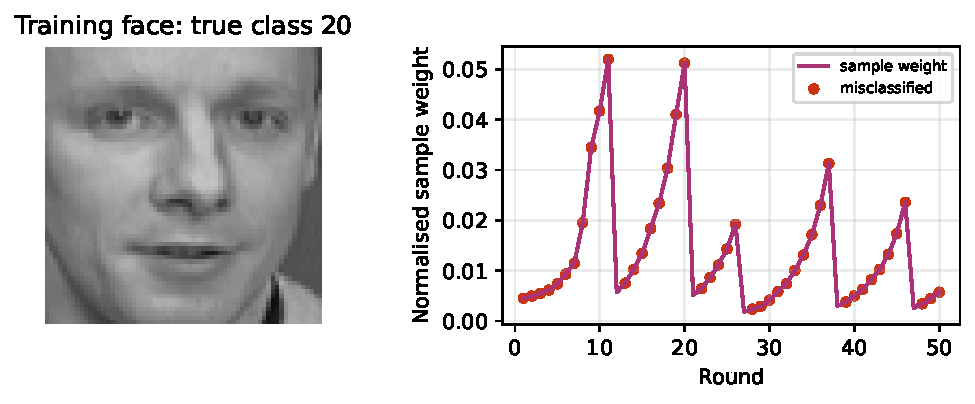
\includegraphics[width=0.88\linewidth]{../figures/boosting_heavy_face.pdf}
\caption{Training source index 204, class 20, receives the largest weight seen in the selected run. Red points mark rounds that misclassify it.}
\label{fig:heavy}
\end{figure}

The face in Figure~\ref{fig:heavy} is misclassified in 45 of 50 rounds and reaches weight 0.0520. Its weight repeatedly rises after a miss and falls when a learner gets it right. That is useful when a rare but valid face needs attention. Here, repeated attention to a few difficult views also leaves too little capacity for the rest of the 40-way problem.

\subsection{Response to the missing centre}
\begin{table}[t]
\centering
\caption{Frozen models on clean and masked test sets. The last column is mean winning probability or vote fraction.}
\label{tab:allmask}
\scriptsize
\begin{tabular}{llrr}
\toprule
Set & Model & Accuracy & Win share\\
\midrule
\multirow{3}{*}{Clean} & Tree &53.75&96.25\\
& Bagging &85.00&41.13\\
& Boosting &28.75&10.69\\
\midrule
\multirow{3}{*}{Masked} & Tree &18.75&100.00\\
& Bagging &68.75&27.18\\
& Boosting &37.50&9.77\\
\bottomrule
\end{tabular}
\end{table}

\begin{figure}[t]
\centering
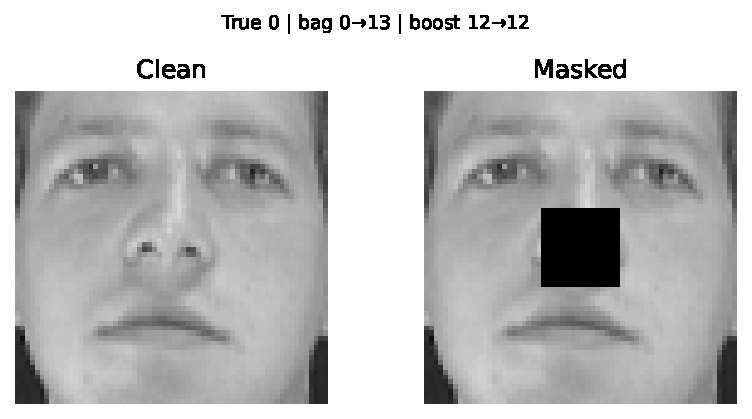
\includegraphics[width=0.72\linewidth]{../figures/bag_boost_mask_response.pdf}
\caption{A test face where the two ensembles react differently to the mask.}
\label{fig:response}
\end{figure}

For source face 6, bagging is correct on the clean image (class 0) but moves to class 13 after masking. Boosting predicts class 12 both times. Bagging's deep trees use many local pixel tests, so removing a central block changes several paths. The shallow boosted trees are less responsive to that block, but their stable answer is still wrong. Stability to a change is not useful by itself if the original rule is biased.

\section{Bias and variance as measurements}
\subsection{Resampling protocol}
I kept the 80 clean test faces fixed. For each of 30 repetitions, I sampled six positions with replacement from each identity's original six training faces. I then refit the frozen single tree, the selected 100-tree bagged model, and the selected 50-round boost without tuning again. For a test face, $p_r(x_i)$ is the 40-way class vector from repetition $r$. It is a tree probability, a bagging vote fraction, or a normalised SAMME weighted vote. I computed
\begin{align}
\mathrm{Bias}^2&=\frac{1}{N}\sum_i\lVert\bar p(x_i)-e_i\rVert_2^2,\\
\mathrm{Variance}&=\frac{1}{NR}\sum_{i,r}\lVert p_r(x_i)-\bar p(x_i)\rVert_2^2.
\end{align}

\begin{table}[t]
\centering
\caption{Measured quantities across 30 resampled training sets. Accuracy is mean $\pm$ sample standard deviation.}
\label{tab:bvselected}
\scriptsize
\begin{tabular}{lrrr}
\toprule
Model & Bias$^2$ & Variance & Test accuracy\\
\midrule
Tree & 0.3947 & 0.6503 & $47.75\pm4.55$\\
Bagging & 0.4890 & 0.0250 & $79.75\pm2.73$\\
Boosting & 0.9082 & \textbf{0.0185} & $17.38\pm4.85$\\
\bottomrule
\end{tabular}
\end{table}

The single tree has the smallest measured bias but by far the largest variance. Bagging raises bias by 0.0943, yet removes 0.6253 variance and raises mean accuracy by 32 points. Boosting is slightly steadier than bagging, but its bias is 0.9082. Its low variance means it repeats a weak rule consistently; it does not mean the rule is good.

\subsection{What depth changes}
I repeated the calculation at depth 2, depth 8, and unlimited depth. At each depth I also built a 100-tree bagged model. The leaf size stayed at the frozen value of two.

\begin{table}[H]
\centering
\caption{Depth study over the same 30 resamples. $L$ is the mean occupied leaf count. $D$ is mean pairwise test disagreement among the 100 bagged trees.}
\label{tab:bvdepth}
\scriptsize
\begin{tabular}{rllrrrr}
\toprule
Depth & Model & Bias$^2$ & Var. & Accuracy & $L$ & $D$\\
\midrule
2 & Tree & .9134 & .0417 & 6.13 & 3.07 & .9619\\
2 & Bag & .9276 & .0106 & 15.96 & 3.07 & .9619\\
8 & Tree & .7760 & .1269 & 16.29 & 9.37 & .9252\\
8 & Bag & .8016 & .0176 & 46.58 & 9.37 & .9252\\
\NA & Tree & .3947 & .6503 & 47.75 & 40.00 & .8125\\
\NA & Bag & .4890 & .0250 & 79.75 & 40.00 & .8125\\
\bottomrule
\end{tabular}
\end{table}

\begin{figure}[H]
\centering
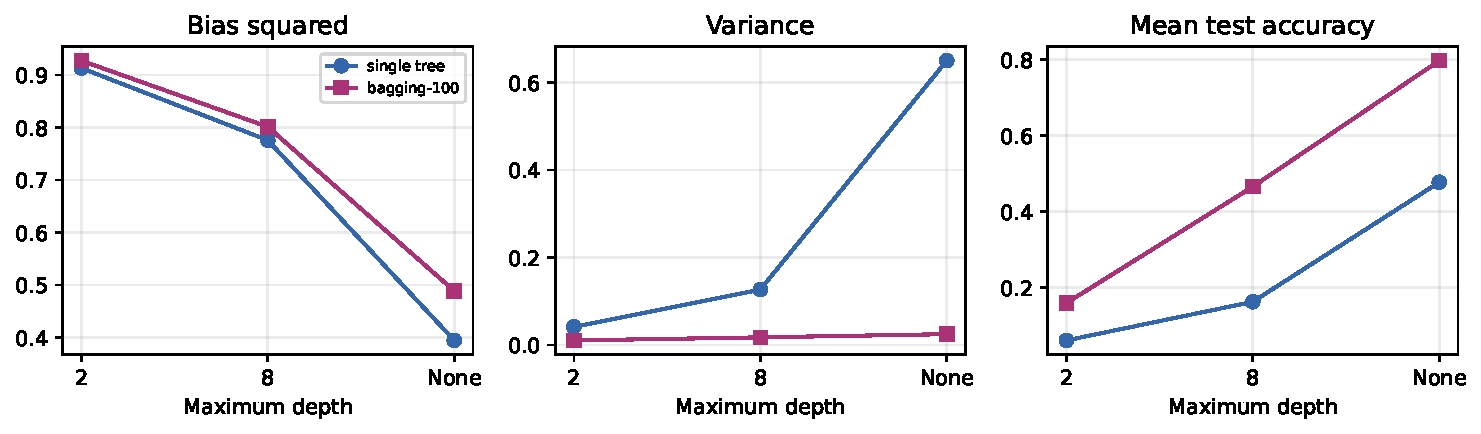
\includegraphics[width=\linewidth]{../figures/depth_bias_variance.pdf}
\caption{Bias squared, variance, and mean clean test accuracy as depth increases.}
\label{fig:depthbv}
\end{figure}

Depth lowers bias and opens more occupied leaves, but the fitted tree becomes more dependent on the sampled faces. Single-tree variance rises from 0.0417 at depth two to 0.6503 without a depth limit. Bagging removes 0.0310, 0.1093, and 0.6253 variance at the three depths. It helps little at depth two because averaging cannot create class distinctions that the three-leaf trees never learned.
The singleton-leaf fraction is zero at all three depths because the frozen minimum leaf size is two.

The deepest setting gives the largest accuracy gain here: 32.00 points, compared with 30.29 at depth eight and 9.83 at depth two. That is a measured result for this split, not a rule that the deepest tree must always gain most. Its trees actually have lower pairwise disagreement (0.8125) than the shallower ensembles. The larger gain comes from combining low-bias trees whose individual predictions move strongly across resamples. Leaf capacity, disagreement, bias, and variance all matter together.

\subsection{Final comparison}
\begin{table}[H]
\centering
\caption{The three selected models. Clean and masked columns use the single fixed split; bias and variance use the 30 resampled fits.}
\label{tab:final}
\scriptsize
\begin{tabular}{lrrrr}
\toprule
Model & Clean & Masked & Bias$^2$ & Variance\\
\midrule
Tree &53.75&18.75&0.3947&0.6503\\
Bagging &85.00&68.75&0.4890&0.0250\\
Boosting &28.75&37.50&0.9082&0.0185\\
\bottomrule
\end{tabular}
\end{table}

Bagging is the most stable useful model: its variance is close to boosting's, but its clean accuracy is much higher. The tree is most sensitive to the missing region, losing 35 points. Bagging loses 16.25 points. Boosting rises by 8.75 points after masking, but both of its scores are low; this is not meaningful resistance to missing data. The lowest-variance model is therefore not the model with the best test accuracy. Bias can dominate, as it does for boosting here.

\section{Reproduction notes}
The archive contains the exact split in CSV and NPZ form, the JSON configuration, every table used here, plot files, the final run log, and the complete source. Running
\begin{quote}\small
\texttt{python src/run\_experiments.py --repetitions 30 --jobs 8}
\end{quote}
from the repository root rebuilds the results. Parallel work is only across independent bootstrap fits or independent repetitions. Every random draw has an explicit seed, so changing the worker count does not change the saved numbers.

\section{Conclusion}
The main result is quite concrete. A deep tree is useful for 40-way face recognition, but its exact rules move a lot when the six training images per person are resampled. Bagging keeps the useful depth and averages away much of that movement. Shallow trees are steady but cannot separate enough identities, so bagging cannot rescue them. The selected SAMME model is also steady, but it spends too much weight on a small set of difficult faces and retains high bias. On this split, the 100-tree bagged model is the best fit to both the clean task and the missing-centre test.

{\small
\begin{thebibliography}{2}
\bibitem{samme} J. Zhu, H. Zou, S. Rosset, and T. Hastie. Multi-class AdaBoost. \textit{Statistics and Its Interface}, 2009.
\bibitem{olivetti} F. S. Samaria and A. C. Harter. Parameterisation of a stochastic model for human face identification. \textit{Proceedings of the IEEE Workshop on Applications of Computer Vision}, 1994.
\end{thebibliography}}

\end{document}
